\chapter{Pure Data Patches}\label{ap:pd_patches}
\Todo{make the patches more readable and replace the pics}

\section{Filter Based Additive Synthesis}
\begin{figure}[H]
  \centering
    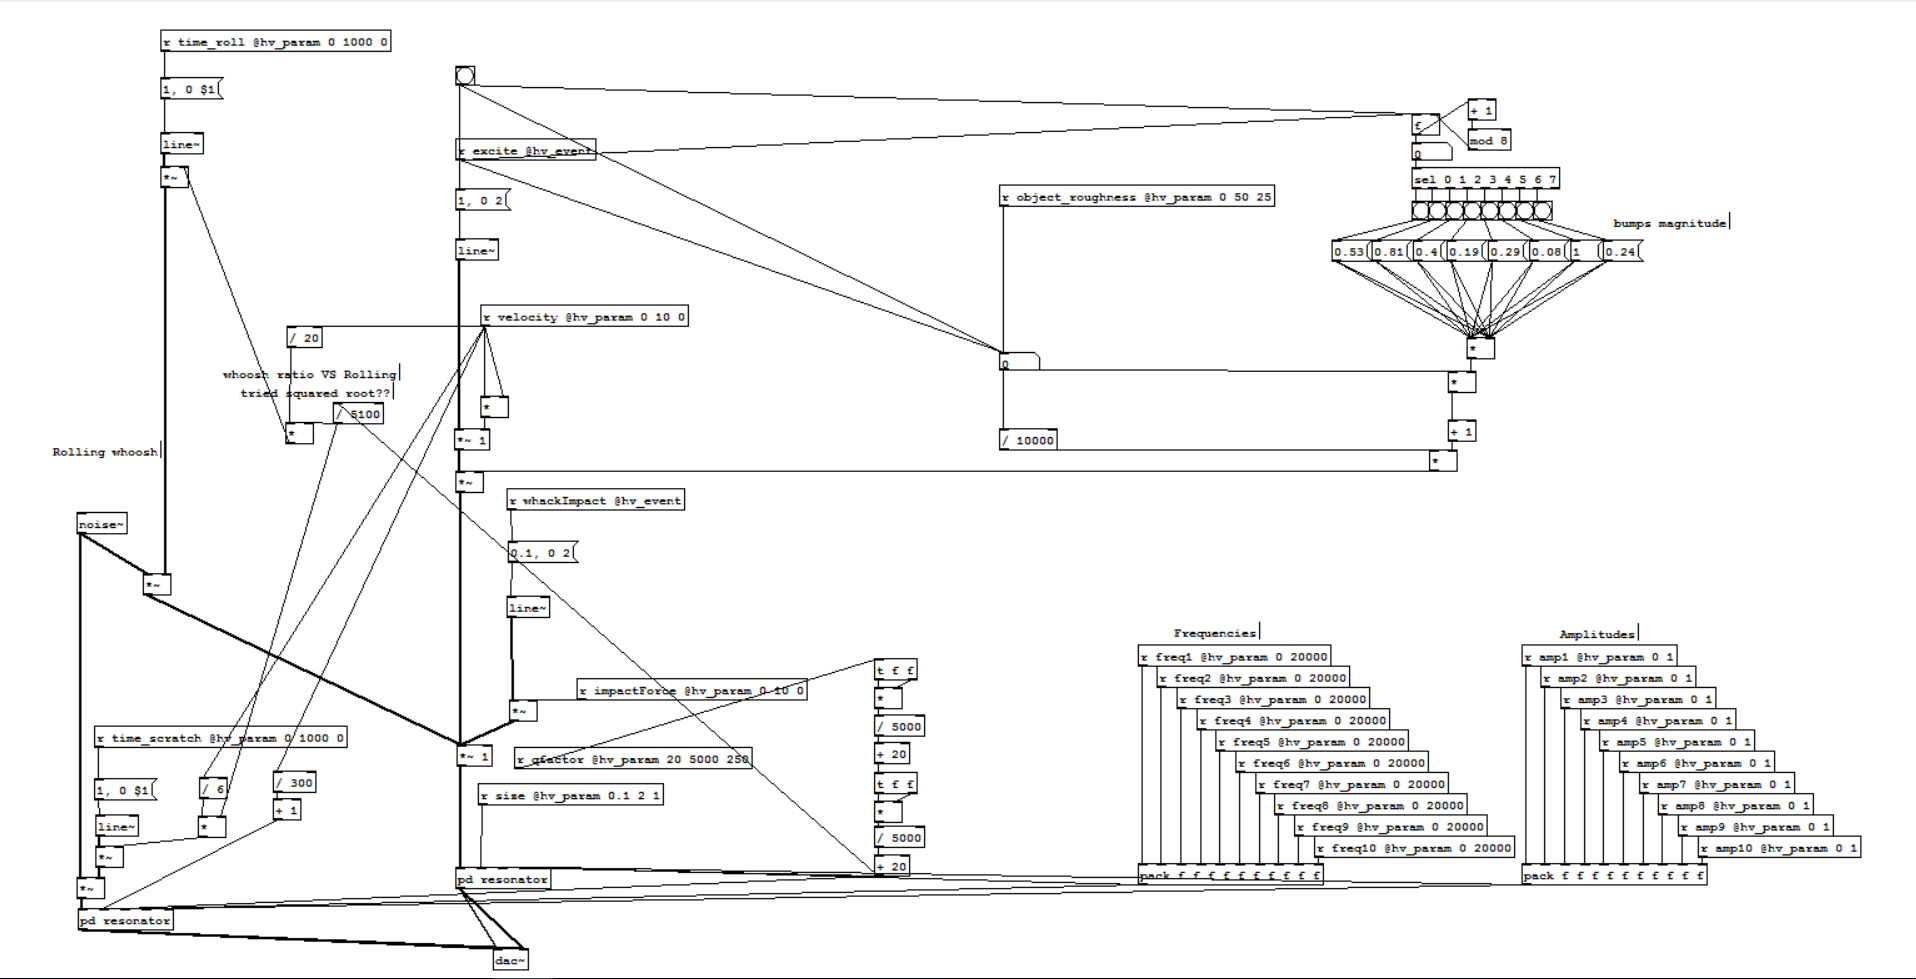
\includegraphics[width=\textwidth]{PdPatches/FBmain.PNG}
      \caption{The main Pure Data patch for the filter-based additive synthesis.}
      \label{fig:FBmain}
\end{figure}

\begin{figure}[H]
  \centering
    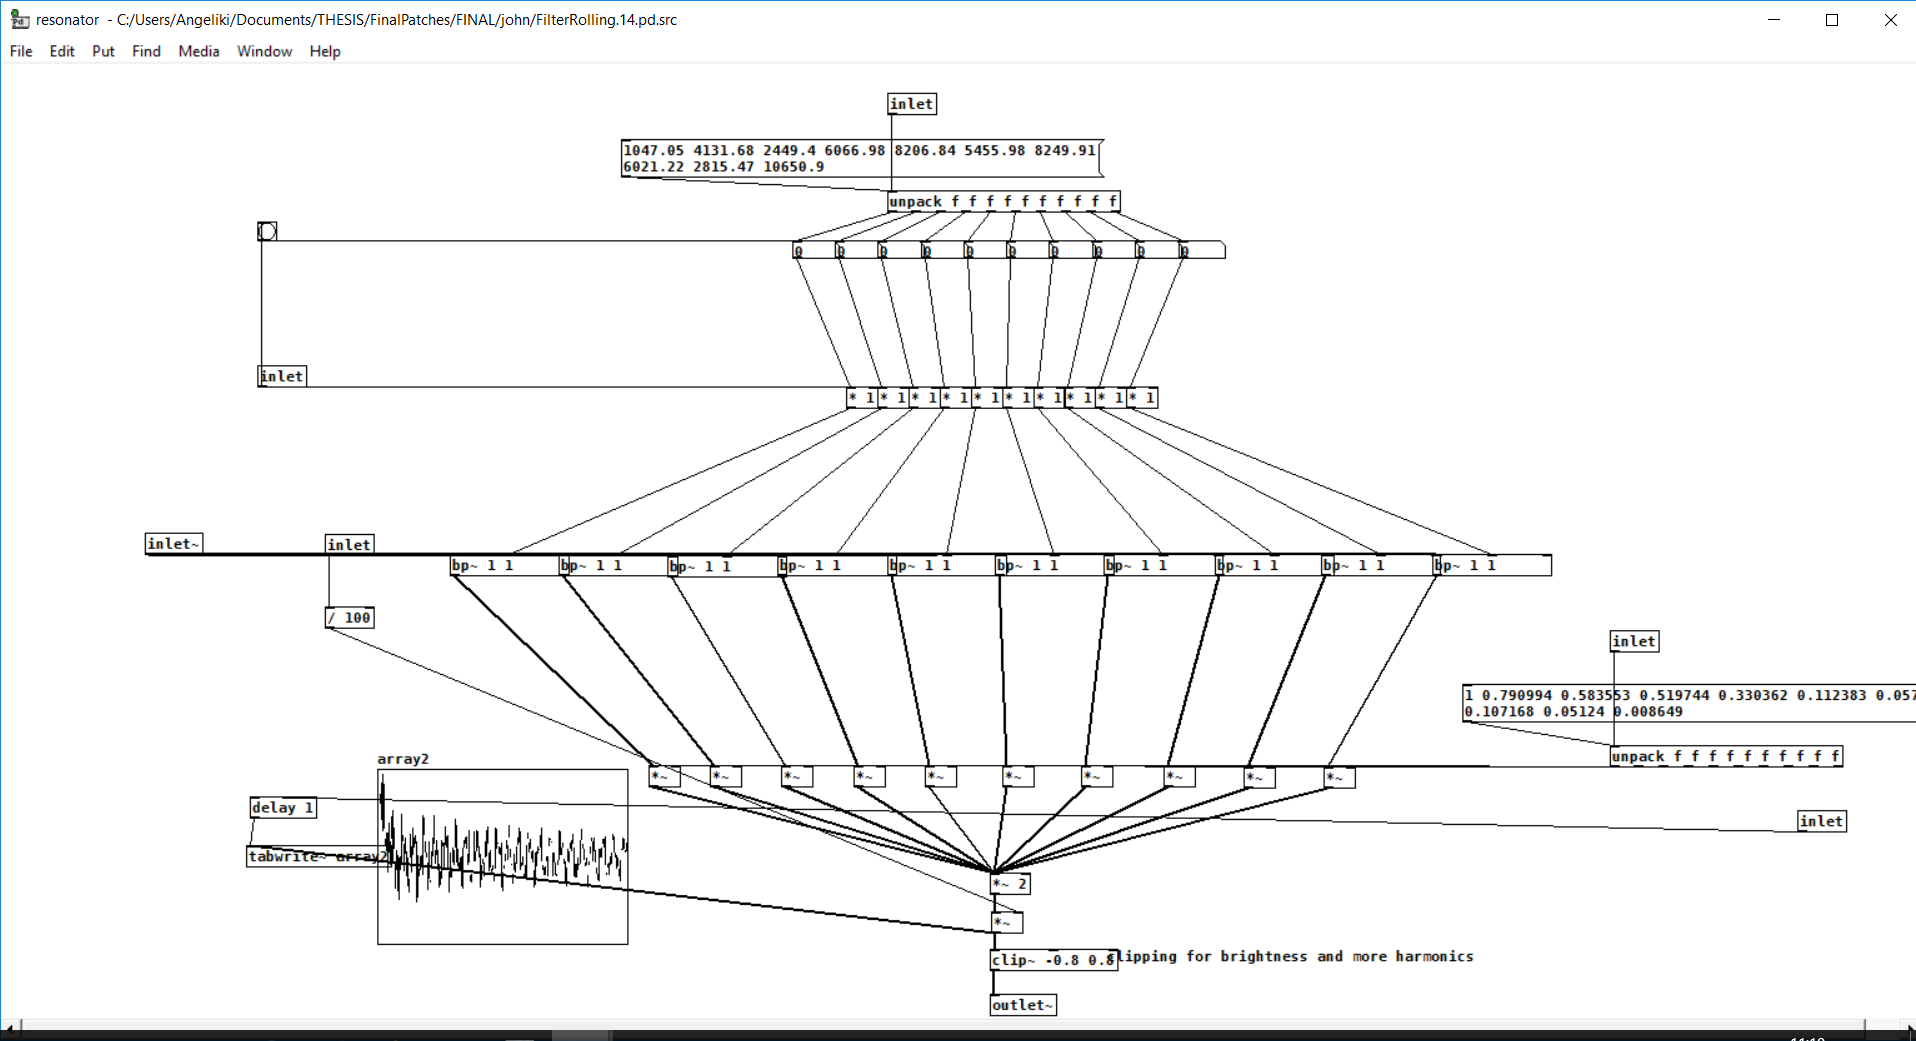
\includegraphics[width=\textwidth]{PdPatches/FBresonator.PNG}
      \caption{The resonator Pure Data patch for the filter-based additive synthesis.}
      \label{fig:FBres}
\end{figure}

\section{Sinusoidal Additive Synthesis}

\begin{figure}[H]
  \centering
    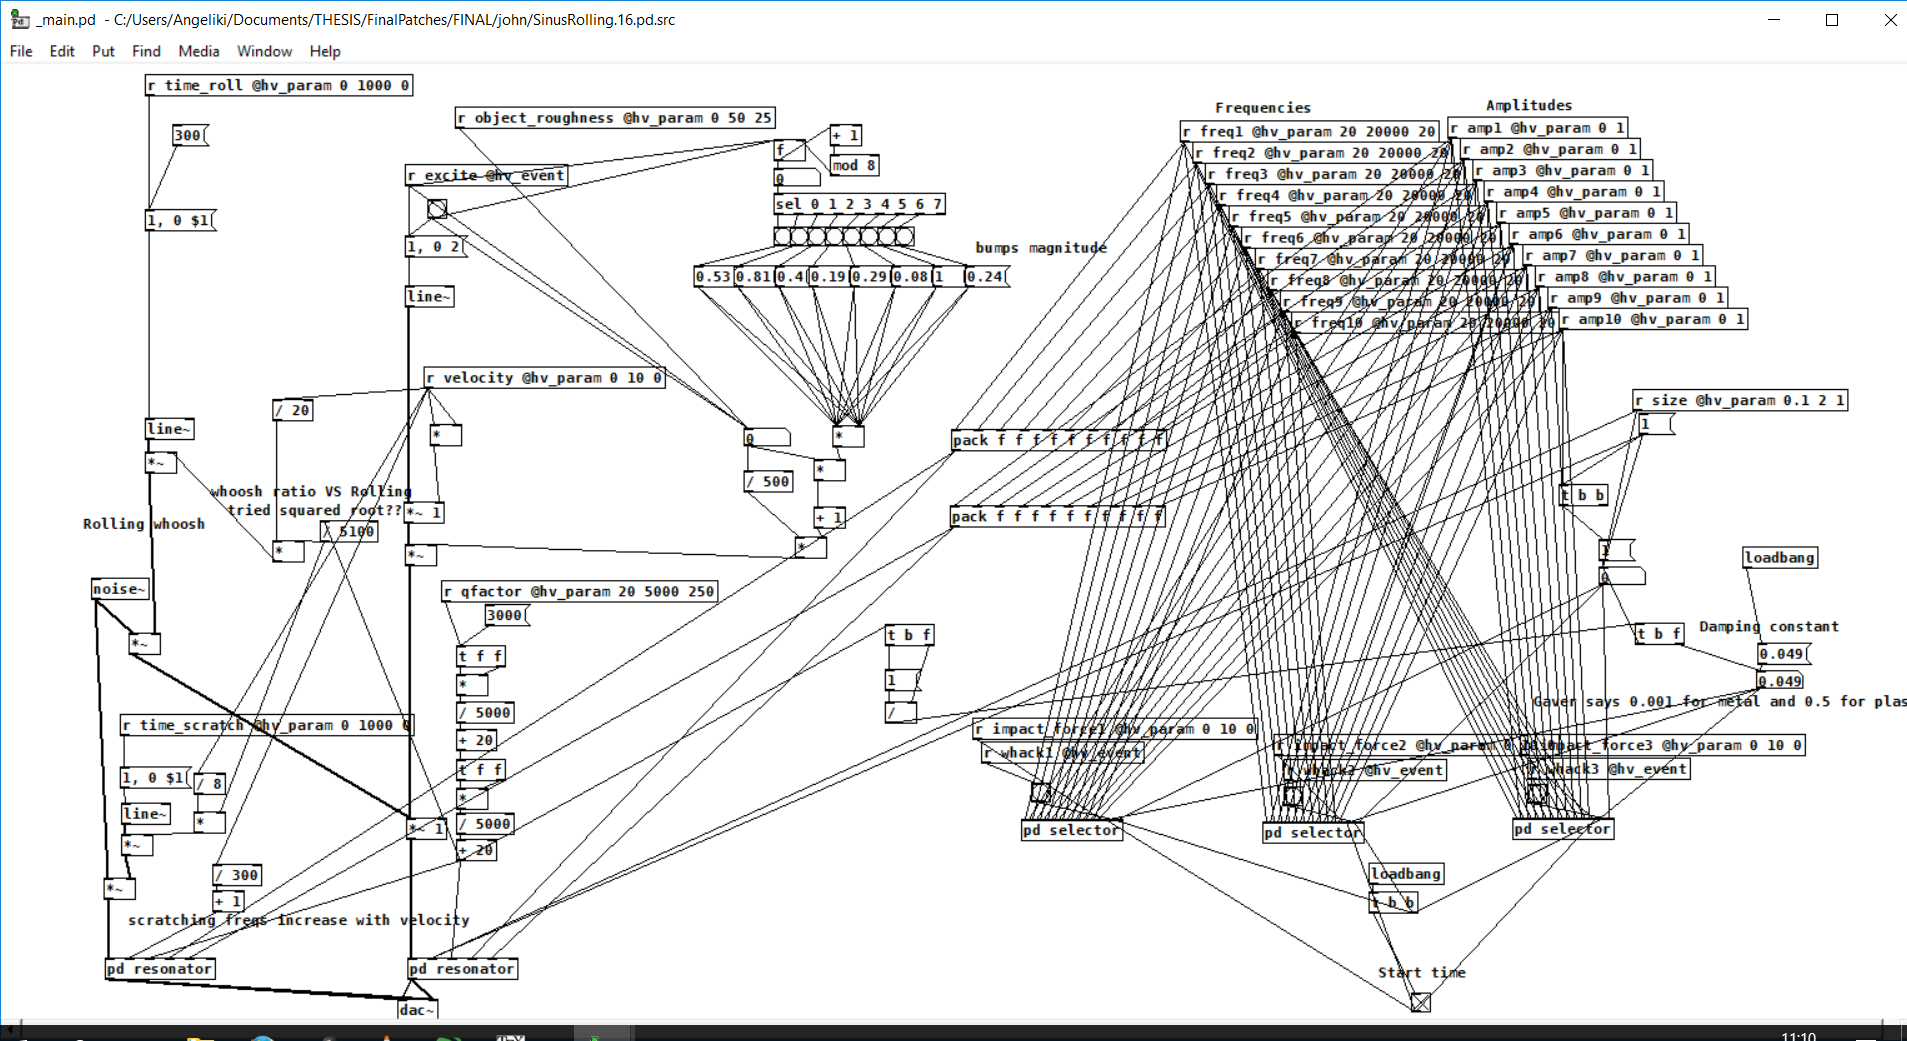
\includegraphics[width=\textwidth]{PdPatches/Smain.PNG}
      \caption{The main Pure Data patch for the sinusoidal additive synthesis.}
      \label{fig:Smain}
\end{figure}

\begin{figure}[H]
  \centering
    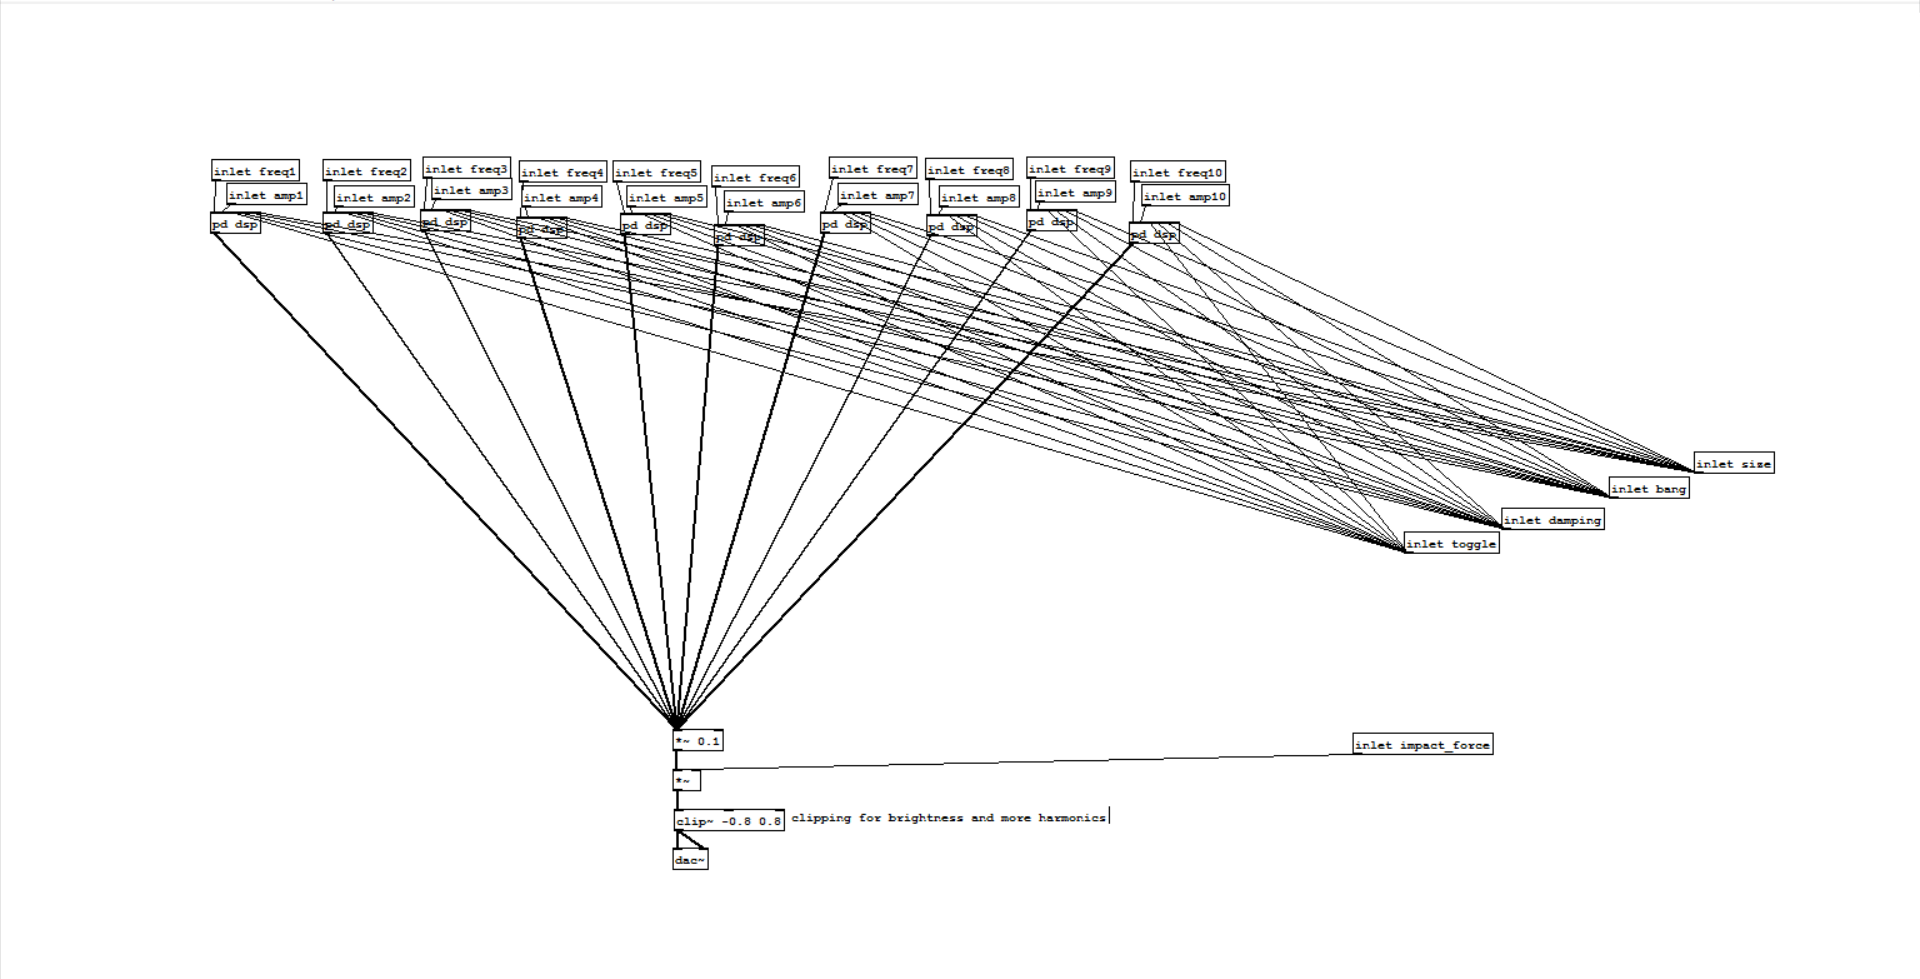
\includegraphics[width=\textwidth]{PdPatches/Sselector.PNG}
      \caption{The selector Pure Data patch for the filter-based additive synthesis.}
      \label{fig:Ssel}
\end{figure}

\begin{figure}[H]
  \centering
    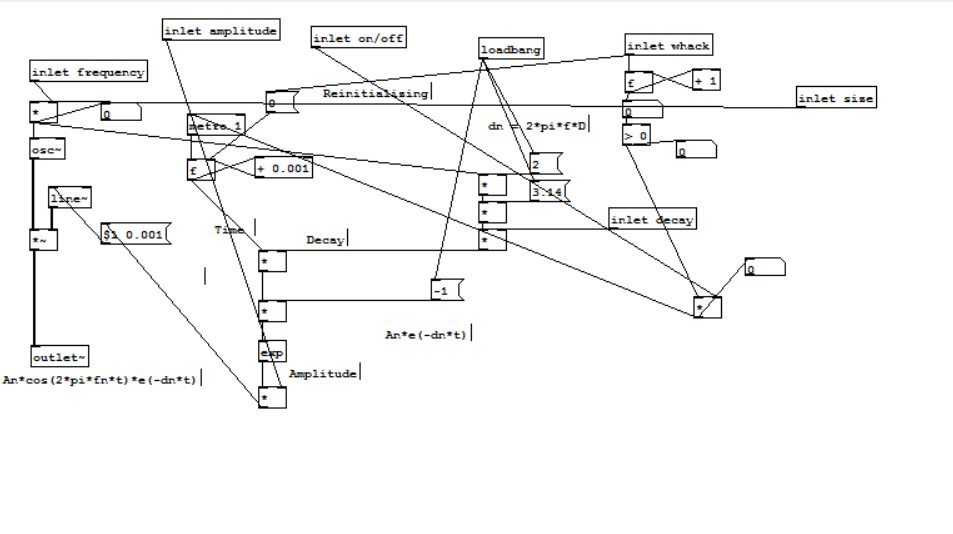
\includegraphics[width=\textwidth]{PdPatches/Sdsp.PNG}
      \caption{The dsp Pure Data patch for the filter-based additive synthesis.}
      \label{fig:Sdsp}
\end{figure}

\chapter{Instructions for the Subjective Experiments}
\Todo{should we include it or not?}

\chapter{Spectrograms}\label{ap:spectrograms}
\section*{Plastic bowl}

\begin{figure}[H]
    \centering
    \begin{subfigure}[b]{0.25\textwidth}
        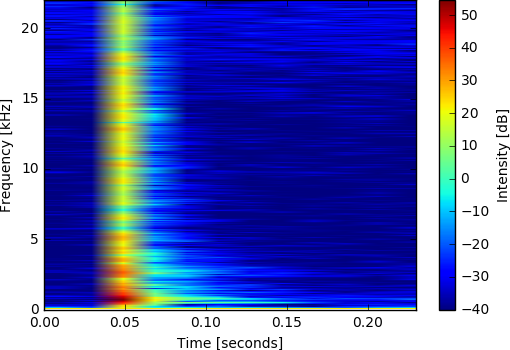
\includegraphics[width=\textwidth]{specs/spectrograms/plasticbowlTOP_rec.png}
    \end{subfigure}%
    ~ %add desired spacing between images, e. g. ~, \quad, \qquad, \hfill etc. 
      %(or a blank line to force the subfigure onto a new line)
    \begin{subfigure}[b]{0.25\textwidth}
        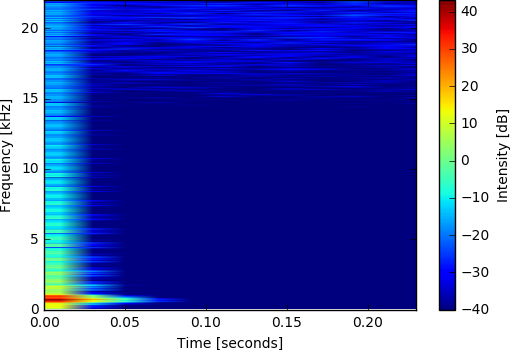
\includegraphics[width=\textwidth]{specs/spectrograms/plasticbowlTOP_sin.png}
    \end{subfigure}%
    ~ %add desired spacing between images, e. g. ~, \quad, \qquad, \hfill etc. 
      %(or a blank line to force the subfigure onto a new line)
    \begin{subfigure}[b]{0.25\textwidth}
        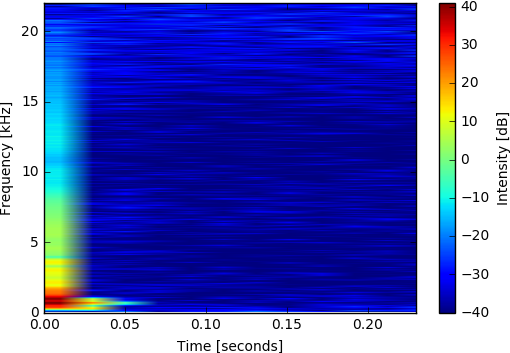
\includegraphics[width=\textwidth]{specs/spectrograms/plasticbowlTOP_fb.png}
    \end{subfigure}%
    %add desired spacing between images, e. g. ~, \quad, \qquad, \hfill etc. 
      %(or a blank line to force the subfigure onto a new line)
      
    \begin{subfigure}[b]{0.25\textwidth}
        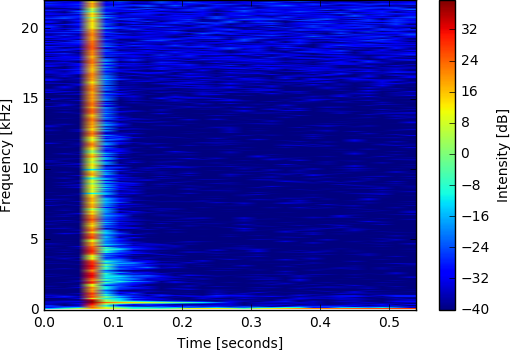
\includegraphics[width=\textwidth]{specs/spectrograms/plasticbowlBODY_rec.png}
    \end{subfigure}%
    ~ %add desired spacing between images, e. g. ~, \quad, \qquad, \hfill etc. 
      %(or a blank line to force the subfigure onto a new line)
    \begin{subfigure}[b]{0.25\textwidth}
        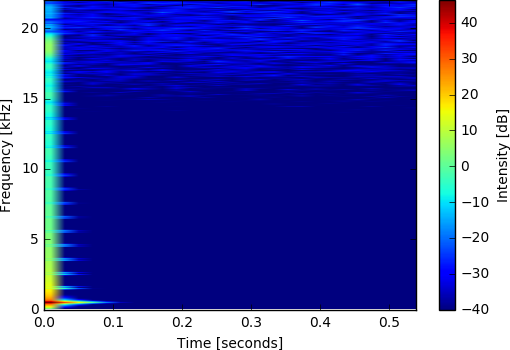
\includegraphics[width=\textwidth]{specs/spectrograms/plasticbowlBODY_sin.png}
    \end{subfigure}%
    ~ %add desired spacing between images, e. g. ~, \quad, \qquad, \hfill etc. 
      %(or a blank line to force the subfigure onto a new line)
    \begin{subfigure}[b]{0.25\textwidth}
        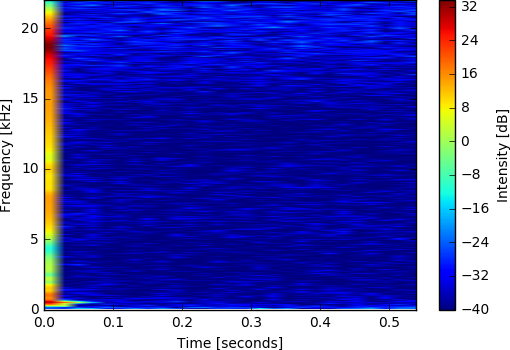
\includegraphics[width=\textwidth]{specs/spectrograms/plasticbowlBODY_fb.png}
    \end{subfigure}%
    %add desired spacing between images, e. g. ~, \quad, \qquad, \hfill etc. 
      %(or a blank line to force the subfigure onto a new line)
      
    \begin{subfigure}[b]{0.25\textwidth}
        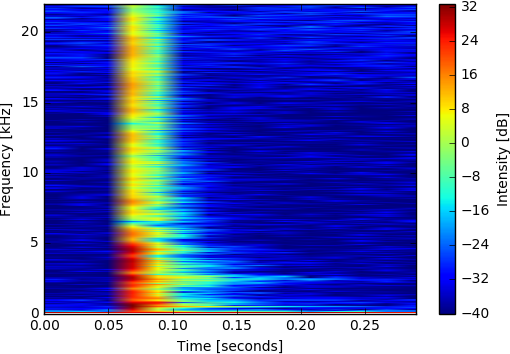
\includegraphics[width=\textwidth]{specs/spectrograms/plasticbowlBOTTOM_rec.png}
    \end{subfigure}%
    ~ %add desired spacing between images, e. g. ~, \quad, \qquad, \hfill etc. 
      %(or a blank line to force the subfigure onto a new line)
    \begin{subfigure}[b]{0.25\textwidth}
        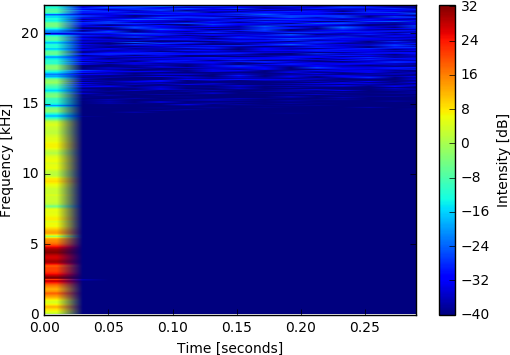
\includegraphics[width=\textwidth]{specs/spectrograms/plasticbowlBOTTOM_sin.png}
    \end{subfigure}%
    ~ %add desired spacing between images, e. g. ~, \quad, \qquad, \hfill etc. 
      %(or a blank line to force the subfigure onto a new line)
    \begin{subfigure}[b]{0.25\textwidth}
        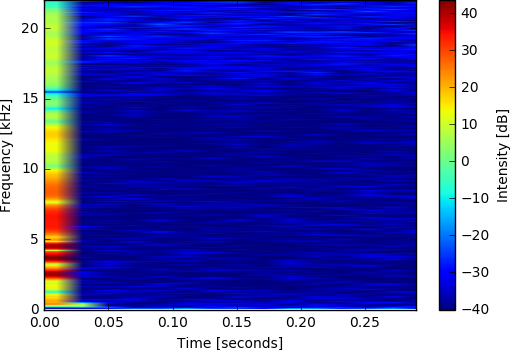
\includegraphics[width=\textwidth]{specs/spectrograms/plasticbowlBOTTOM_fb.png}
    \end{subfigure}%
\end{figure}

\section*{Wooden mortar}

\begin{figure}[H]
    \centering
    \begin{subfigure}[b]{0.25\textwidth}
        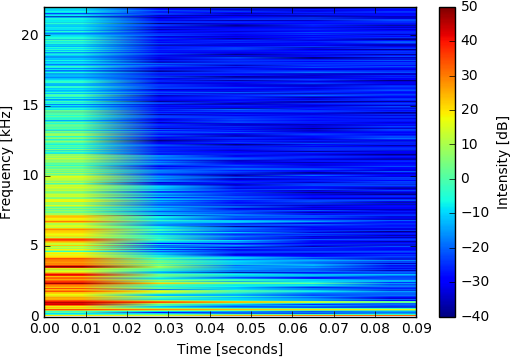
\includegraphics[width=\textwidth]{specs/spectrograms/mortarTOP_rec.png}
    \end{subfigure}%
    ~ %add desired spacing between images, e. g. ~, \quad, \qquad, \hfill etc. 
      %(or a blank line to force the subfigure onto a new line)
    \begin{subfigure}[b]{0.25\textwidth}
        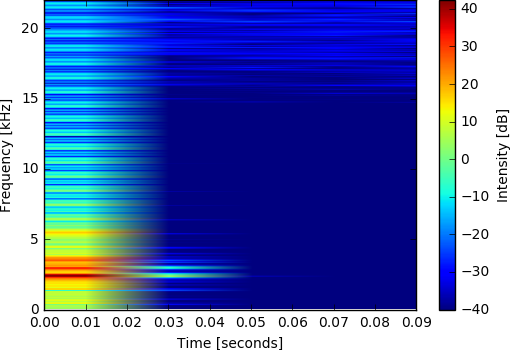
\includegraphics[width=\textwidth]{specs/spectrograms/mortarTOP_sin.png}
    \end{subfigure}%
    ~ %add desired spacing between images, e. g. ~, \quad, \qquad, \hfill etc. 
      %(or a blank line to force the subfigure onto a new line)
    \begin{subfigure}[b]{0.25\textwidth}
        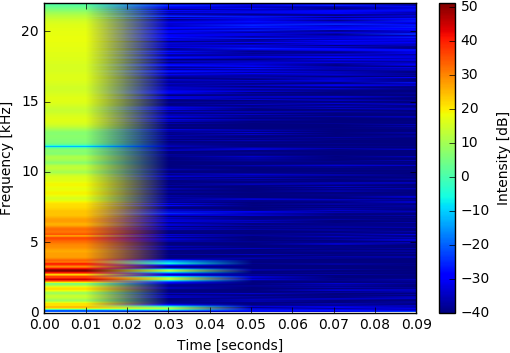
\includegraphics[width=\textwidth]{specs/spectrograms/mortarTOP_fb.png}
    \end{subfigure}%
    %add desired spacing between images, e. g. ~, \quad, \qquad, \hfill etc. 
      %(or a blank line to force the subfigure onto a new line)
      
    \begin{subfigure}[b]{0.25\textwidth}
        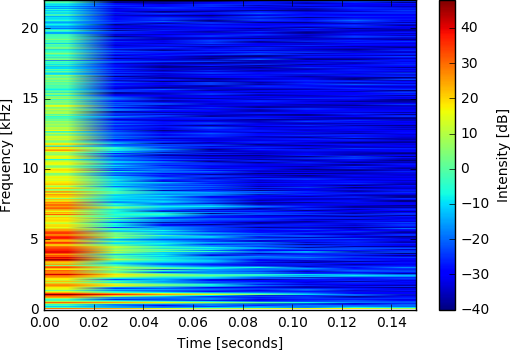
\includegraphics[width=\textwidth]{specs/spectrograms/mortarBODYUPPER_rec.png}
    \end{subfigure}%
    ~ %add desired spacing between images, e. g. ~, \quad, \qquad, \hfill etc. 
      %(or a blank line to force the subfigure onto a new line)
    \begin{subfigure}[b]{0.25\textwidth}
        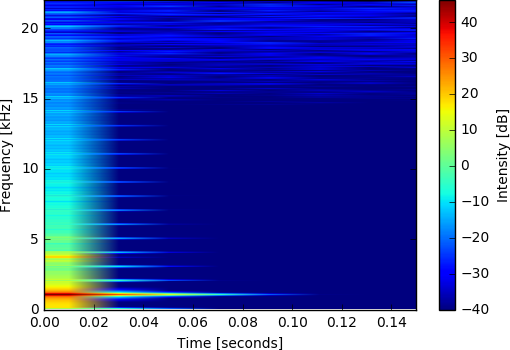
\includegraphics[width=\textwidth]{specs/spectrograms/mortarBODYUPPER_sin.png}
    \end{subfigure}%
    ~ %add desired spacing between images, e. g. ~, \quad, \qquad, \hfill etc. 
      %(or a blank line to force the subfigure onto a new line)
    \begin{subfigure}[b]{0.25\textwidth}
        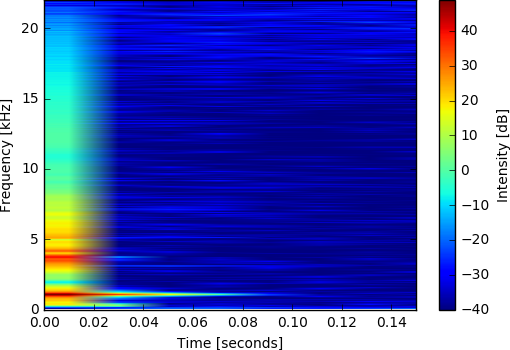
\includegraphics[width=\textwidth]{specs/spectrograms/mortarBODYUPPER_fb.png}
    \end{subfigure}%
    \end{figure}
    %add desired spacing between images, e. g. ~, \quad, \qquad, \hfill etc. 
      %(or a blank line to force the subfigure onto a new line)
\begin{figure}
	\centering    
    \begin{subfigure}[b]{0.25\textwidth}
        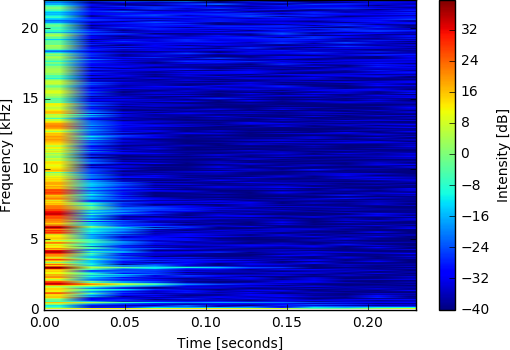
\includegraphics[width=\textwidth]{specs/spectrograms/mortarBODYLOWER_rec.png}
    \end{subfigure}%
    ~ %add desired spacing between images, e. g. ~, \quad, \qquad, \hfill etc. 
      %(or a blank line to force the subfigure onto a new line)
    \begin{subfigure}[b]{0.25\textwidth}
        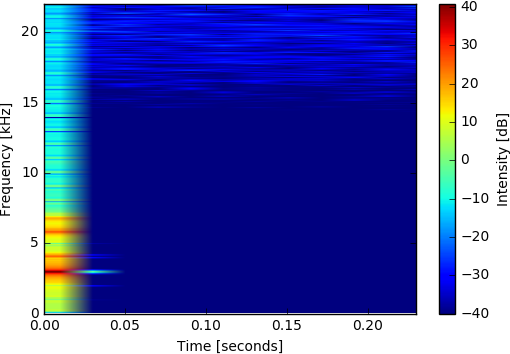
\includegraphics[width=\textwidth]{specs/spectrograms/mortarBODYLOWER_sin.png}
    \end{subfigure}%
    ~ %add desired spacing between images, e. g. ~, \quad, \qquad, \hfill etc. 
      %(or a blank line to force the subfigure onto a new line)
    \begin{subfigure}[b]{0.25\textwidth}
        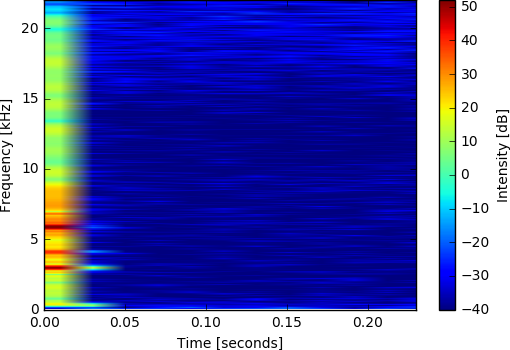
\includegraphics[width=\textwidth]{specs/spectrograms/mortarBODYLOWER_fb.png}
    \end{subfigure}%
    %add desired spacing between images, e. g. ~, \quad, \qquad, \hfill etc. 
      %(or a blank line to force the subfigure onto a new line)
      
    \begin{subfigure}[b]{0.25\textwidth}
        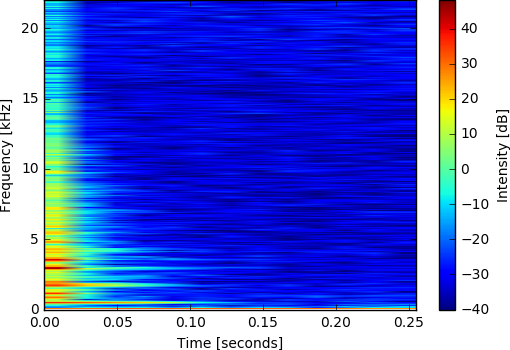
\includegraphics[width=\textwidth]{specs/spectrograms/mortarBOTTOM_rec.png}
    \end{subfigure}%
    ~ %add desired spacing between images, e. g. ~, \quad, \qquad, \hfill etc. 
      %(or a blank line to force the subfigure onto a new line)
    \begin{subfigure}[b]{0.25\textwidth}
        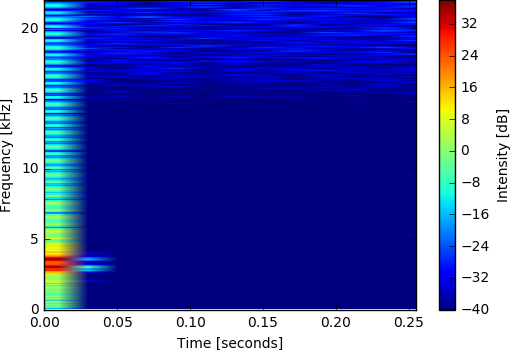
\includegraphics[width=\textwidth]{specs/spectrograms/mortarBOTTOM_sin.png}
    \end{subfigure}%
    ~ %add desired spacing between images, e. g. ~, \quad, \qquad, \hfill etc. 
      %(or a blank line to force the subfigure onto a new line)
    \begin{subfigure}[b]{0.25\textwidth}
        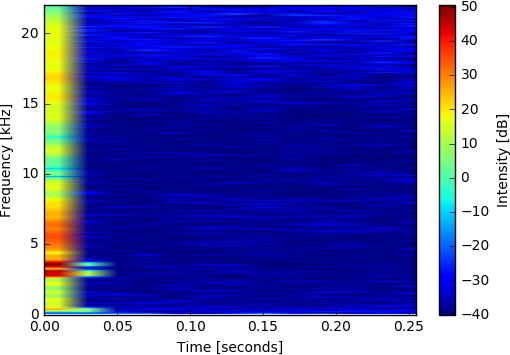
\includegraphics[width=\textwidth]{specs/spectrograms/mortarBOTTOM_fb.png}
    \end{subfigure}%
    \label{fig:spectrograms}
\end{figure}

\section*{Ceramic plate}

\begin{figure}[H]
    \centering
    \begin{subfigure}[b]{0.25\textwidth}
        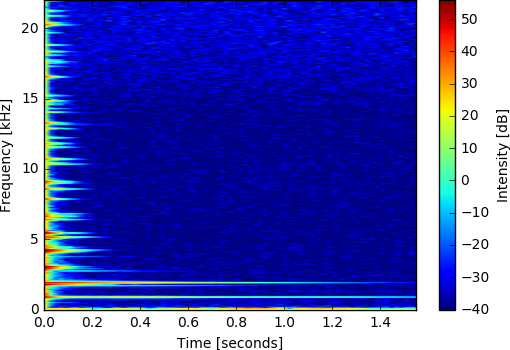
\includegraphics[width=\textwidth]{specs/spectrograms/plateOUTER_rec.png}
    \end{subfigure}%
    ~ %add desired spacing between images, e. g. ~, \quad, \qquad, \hfill etc. 
      %(or a blank line to force the subfigure onto a new line)
    \begin{subfigure}[b]{0.25\textwidth}
        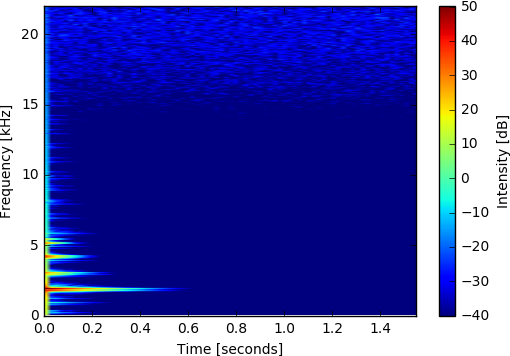
\includegraphics[width=\textwidth]{specs/spectrograms/plateOUTER_sin.png}
    \end{subfigure}%
    ~ %add desired spacing between images, e. g. ~, \quad, \qquad, \hfill etc. 
      %(or a blank line to force the subfigure onto a new line)
    \begin{subfigure}[b]{0.25\textwidth}
        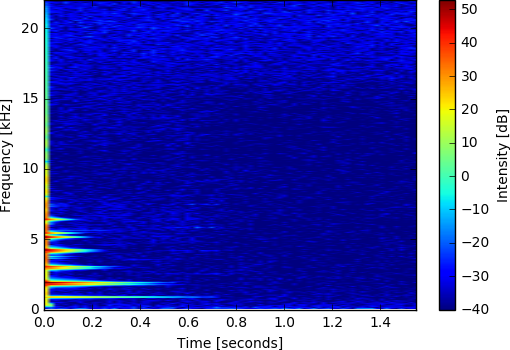
\includegraphics[width=\textwidth]{specs/spectrograms/plateOUTER_fb.png}
    \end{subfigure}%
    %add desired spacing between images, e. g. ~, \quad, \qquad, \hfill etc. 
      %(or a blank line to force the subfigure onto a new line)
      
    \begin{subfigure}[b]{0.25\textwidth}
        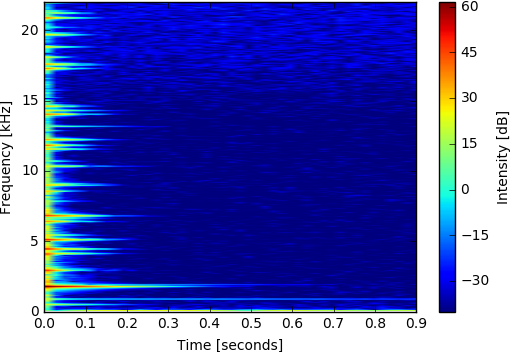
\includegraphics[width=\textwidth]{specs/spectrograms/plateMIDDLE_rec.png}
    \end{subfigure}%
    ~ %add desired spacing between images, e. g. ~, \quad, \qquad, \hfill etc. 
      %(or a blank line to force the subfigure onto a new line)
    \begin{subfigure}[b]{0.25\textwidth}
        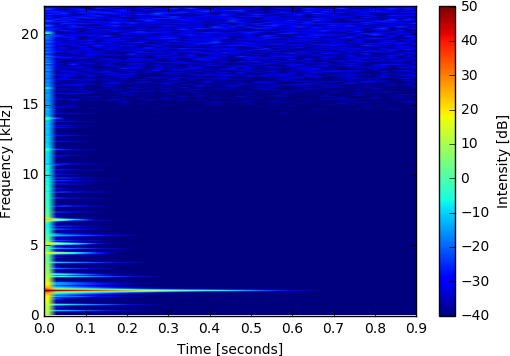
\includegraphics[width=\textwidth]{specs/spectrograms/plateMIDDLE_sin.png}
    \end{subfigure}%
    ~ %add desired spacing between images, e. g. ~, \quad, \qquad, \hfill etc. 
      %(or a blank line to force the subfigure onto a new line)
    \begin{subfigure}[b]{0.25\textwidth}
        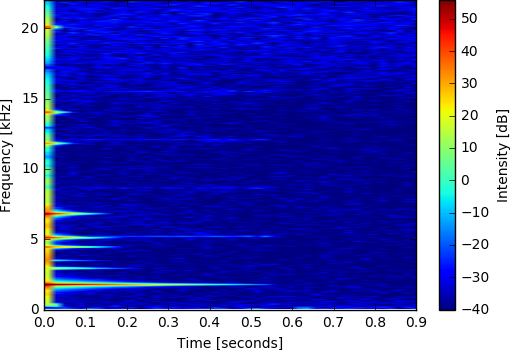
\includegraphics[width=\textwidth]{specs/spectrograms/plateMIDDLE_fb.png}
    \end{subfigure}%
    %add desired spacing between images, e. g. ~, \quad, \qquad, \hfill etc. 
      %(or a blank line to force the subfigure onto a new line)
      
    \begin{subfigure}[b]{0.25\textwidth}
        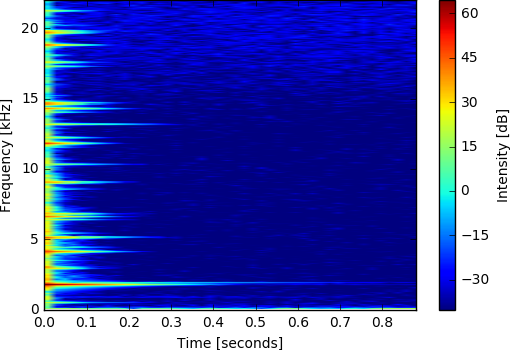
\includegraphics[width=\textwidth]{specs/spectrograms/plateCENTER_rec.png}
    \end{subfigure}%
    ~ %add desired spacing between images, e. g. ~, \quad, \qquad, \hfill etc. 
      %(or a blank line to force the subfigure onto a new line)
    \begin{subfigure}[b]{0.25\textwidth}
        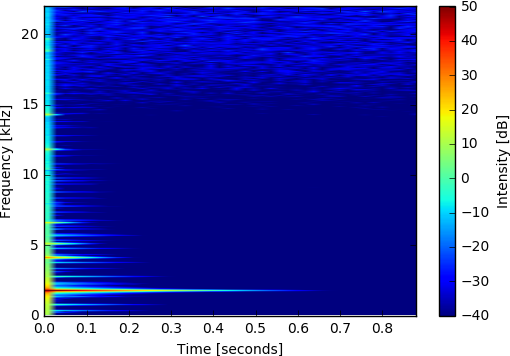
\includegraphics[width=\textwidth]{specs/spectrograms/plateCENTER_sin.png}
    \end{subfigure}%
    ~ %add desired spacing between images, e. g. ~, \quad, \qquad, \hfill etc. 
      %(or a blank line to force the subfigure onto a new line)
    \begin{subfigure}[b]{0.25\textwidth}
        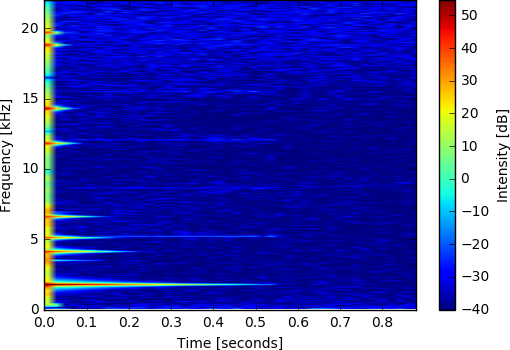
\includegraphics[width=\textwidth]{specs/spectrograms/plateCENTER_fb.png}
    \end{subfigure}%
\end{figure}

\section*{Wine glass}

\begin{figure}[H]
    \centering
    \begin{subfigure}[b]{0.25\textwidth}
        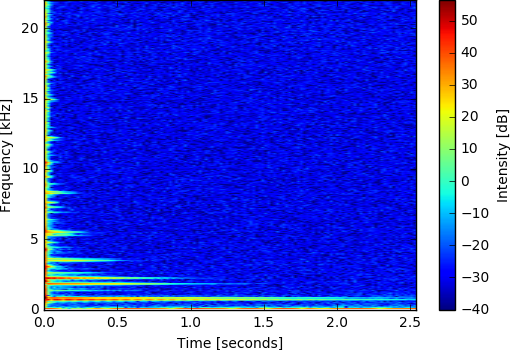
\includegraphics[width=\textwidth]{specs/spectrograms/wineglassTOP_rec.png}
    \end{subfigure}%
    ~ %add desired spacing between images, e. g. ~, \quad, \qquad, \hfill etc. 
      %(or a blank line to force the subfigure onto a new line)
    \begin{subfigure}[b]{0.25\textwidth}
        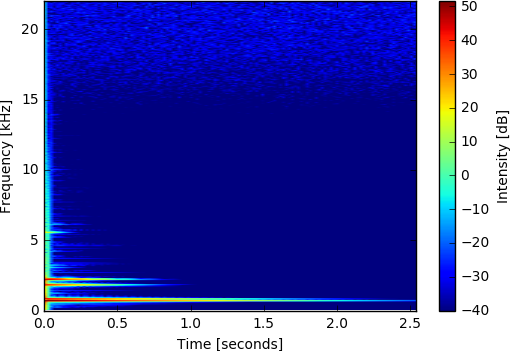
\includegraphics[width=\textwidth]{specs/spectrograms/wineglassTOP_sin.png}
    \end{subfigure}%
    ~ %add desired spacing between images, e. g. ~, \quad, \qquad, \hfill etc. 
      %(or a blank line to force the subfigure onto a new line)
    \begin{subfigure}[b]{0.25\textwidth}
        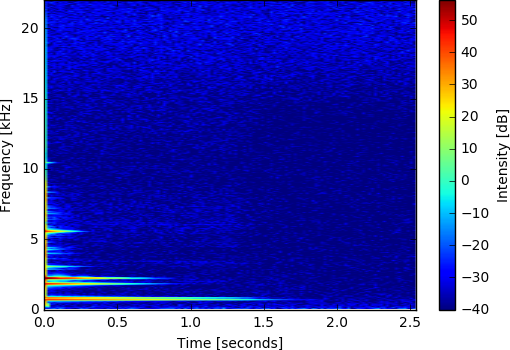
\includegraphics[width=\textwidth]{specs/spectrograms/wineglassTOP_fb.png}
    \end{subfigure}%
    %add desired spacing between images, e. g. ~, \quad, \qquad, \hfill etc. 
      %(or a blank line to force the subfigure onto a new line)
      
    \begin{subfigure}[b]{0.25\textwidth}
        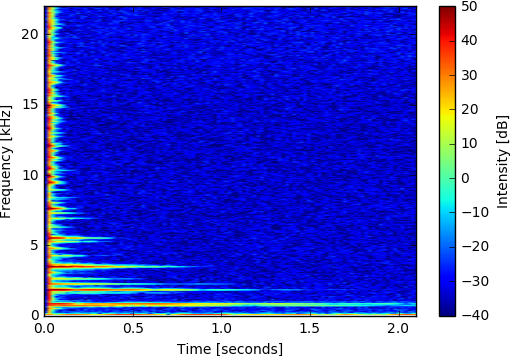
\includegraphics[width=\textwidth]{specs/spectrograms/wineglassBODYUPPER_rec.png}
    \end{subfigure}%
    ~ %add desired spacing between images, e. g. ~, \quad, \qquad, \hfill etc. 
      %(or a blank line to force the subfigure onto a new line)
    \begin{subfigure}[b]{0.25\textwidth}
        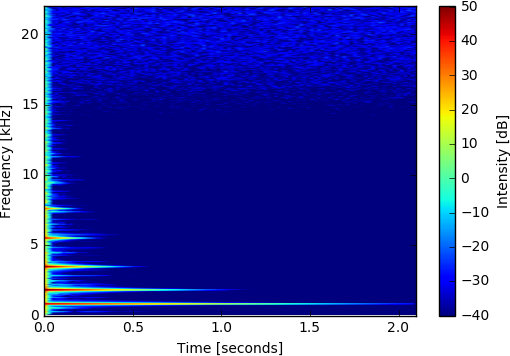
\includegraphics[width=\textwidth]{specs/spectrograms/wineglassBODYUPPER_sin.png}
    \end{subfigure}%
    ~ %add desired spacing between images, e. g. ~, \quad, \qquad, \hfill etc. 
      %(or a blank line to force the subfigure onto a new line)
    \begin{subfigure}[b]{0.25\textwidth}
        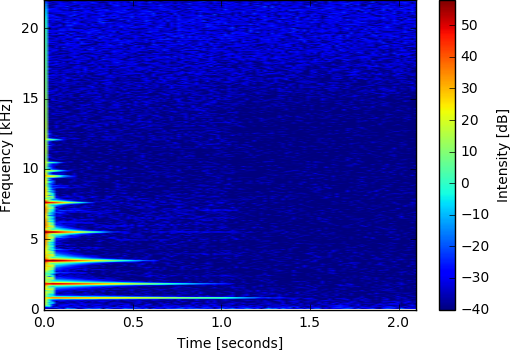
\includegraphics[width=\textwidth]{specs/spectrograms/wineglassBODYUPPER_fb.png}
    \end{subfigure}%
    \end{figure}
    %add desired spacing between images, e. g. ~, \quad, \qquad, \hfill etc. 
      %(or a blank line to force the subfigure onto a new line)
\begin{figure}
	\centering      
    \begin{subfigure}[b]{0.25\textwidth}
        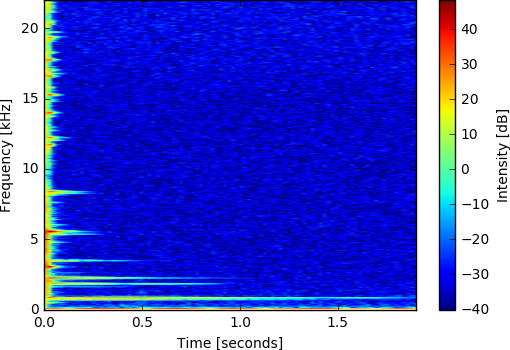
\includegraphics[width=\textwidth]{specs/spectrograms/wineglassBODYLOWER_rec.png}
    \end{subfigure}%
    ~ %add desired spacing between images, e. g. ~, \quad, \qquad, \hfill etc. 
      %(or a blank line to force the subfigure onto a new line)
    \begin{subfigure}[b]{0.25\textwidth}
        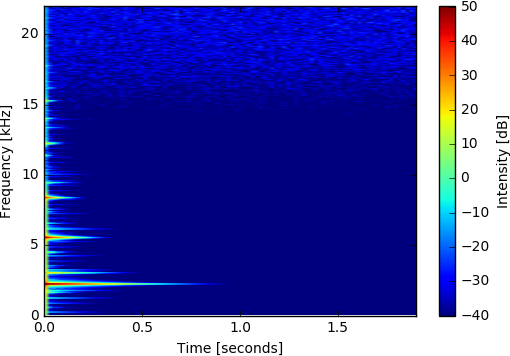
\includegraphics[width=\textwidth]{specs/spectrograms/wineglassBODYLOWER_sin.png}
    \end{subfigure}%
    ~ %add desired spacing between images, e. g. ~, \quad, \qquad, \hfill etc. 
      %(or a blank line to force the subfigure onto a new line)
    \begin{subfigure}[b]{0.25\textwidth}
        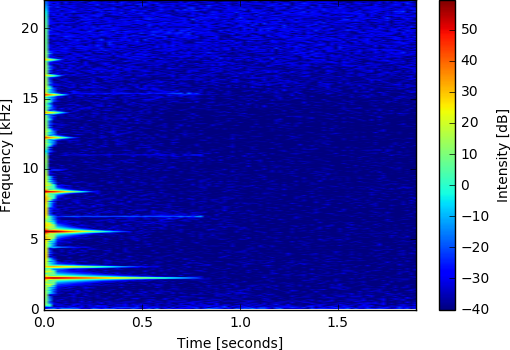
\includegraphics[width=\textwidth]{specs/spectrograms/wineglassBODYLOWER_fb.png}
    \end{subfigure}%
    %add desired spacing between images, e. g. ~, \quad, \qquad, \hfill etc. 
      %(or a blank line to force the subfigure onto a new line)
      
    \begin{subfigure}[b]{0.25\textwidth}
        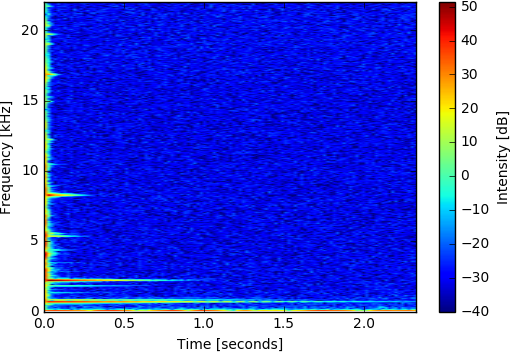
\includegraphics[width=\textwidth]{specs/spectrograms/wineglassSTEM_rec.png}
    \end{subfigure}%
    ~ %add desired spacing between images, e. g. ~, \quad, \qquad, \hfill etc. 
      %(or a blank line to force the subfigure onto a new line)
    \begin{subfigure}[b]{0.25\textwidth}
        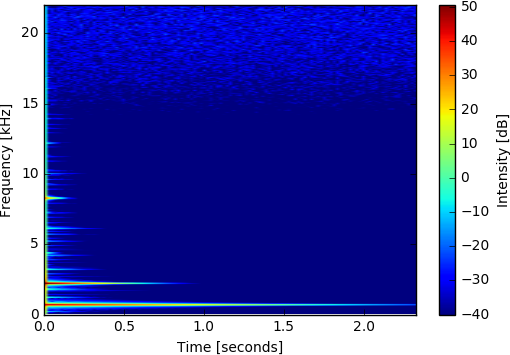
\includegraphics[width=\textwidth]{specs/spectrograms/wineglassSTEM_sin.png}
    \end{subfigure}%
    ~ %add desired spacing between images, e. g. ~, \quad, \qquad, \hfill etc. 
      %(or a blank line to force the subfigure onto a new line)
    \begin{subfigure}[b]{0.25\textwidth}
        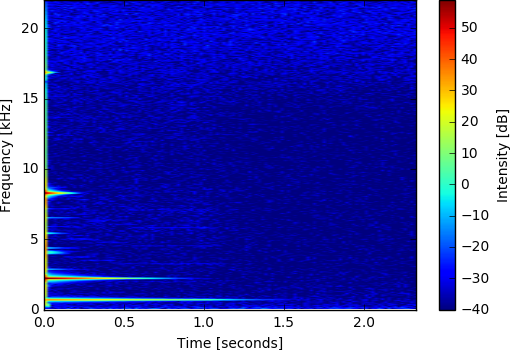
\includegraphics[width=\textwidth]{specs/spectrograms/wineglassSTEM_fb.png}
    \end{subfigure}%
    %add desired spacing between images, e. g. ~, \quad, \qquad, \hfill etc. 
      %(or a blank line to force the subfigure onto a new line)
      
    \begin{subfigure}[b]{0.25\textwidth}
        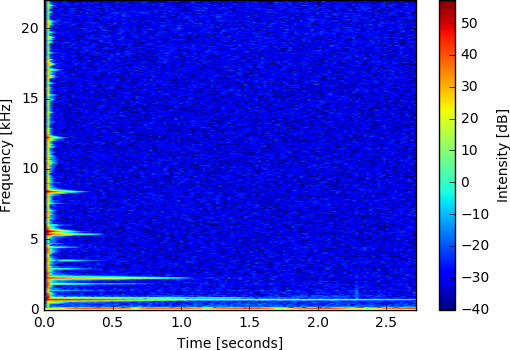
\includegraphics[width=\textwidth]{specs/spectrograms/wineglassFOOT_rec.png}
    \end{subfigure}%
    ~ %add desired spacing between images, e. g. ~, \quad, \qquad, \hfill etc. 
      %(or a blank line to force the subfigure onto a new line)
    \begin{subfigure}[b]{0.25\textwidth}
        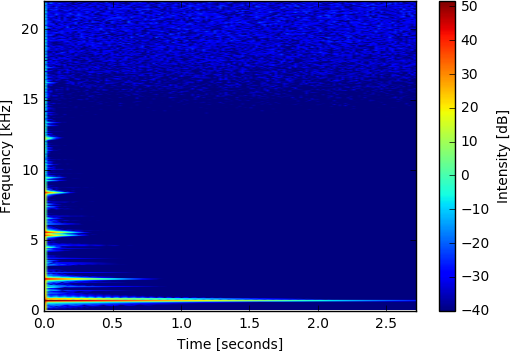
\includegraphics[width=\textwidth]{specs/spectrograms/wineglassFOOT_sin.png}
    \end{subfigure}%
    ~ %add desired spacing between images, e. g. ~, \quad, \qquad, \hfill etc. 
      %(or a blank line to force the subfigure onto a new line)
    \begin{subfigure}[b]{0.25\textwidth}
        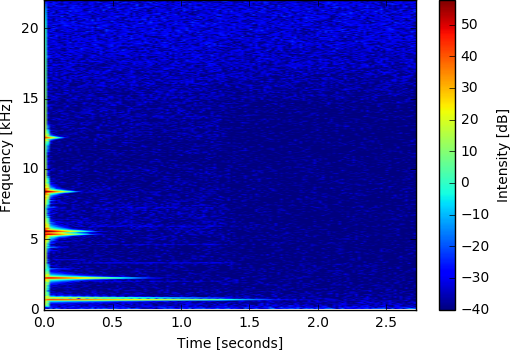
\includegraphics[width=\textwidth]{specs/spectrograms/wineglassFOOT_fb.png}
    \end{subfigure}%
\end{figure}

\section*{Metallic wok}

\begin{figure}[H]
    \centering
    \begin{subfigure}[b]{0.25\textwidth}
        \includegraphics[width=\textwidth]{specs/spectrograms/wokBODYUPPER_rec.png}
    \end{subfigure}%
    ~ %add desired spacing between images, e. g. ~, \quad, \qquad, \hfill etc. 
      %(or a blank line to force the subfigure onto a new line)
    \begin{subfigure}[b]{0.25\textwidth}
        \includegraphics[width=\textwidth]{specs/spectrograms/wokBODYUPPER_sin.png}
    \end{subfigure}%
    ~ %add desired spacing between images, e. g. ~, \quad, \qquad, \hfill etc. 
      %(or a blank line to force the subfigure onto a new line)
    \begin{subfigure}[b]{0.25\textwidth}
        \includegraphics[width=\textwidth]{specs/spectrograms/wokBODYUPPER_fb.png}
    \end{subfigure}%
    %add desired spacing between images, e. g. ~, \quad, \qquad, \hfill etc. 
      %(or a blank line to force the subfigure onto a new line)
      
    \begin{subfigure}[b]{0.25\textwidth}
        \includegraphics[width=\textwidth]{specs/spectrograms/wokBODYLOWER_rec.png}
    \end{subfigure}%
    ~ %add desired spacing between images, e. g. ~, \quad, \qquad, \hfill etc. 
      %(or a blank line to force the subfigure onto a new line)
    \begin{subfigure}[b]{0.25\textwidth}
        \includegraphics[width=\textwidth]{specs/spectrograms/wokBODYLOWER_sin.png}
    \end{subfigure}%
    ~ %add desired spacing between images, e. g. ~, \quad, \qquad, \hfill etc. 
      %(or a blank line to force the subfigure onto a new line)
    \begin{subfigure}[b]{0.25\textwidth}
        \includegraphics[width=\textwidth]{specs/spectrograms/wokBODYLOWER_fb.png}
    \end{subfigure}%
    %add desired spacing between images, e. g. ~, \quad, \qquad, \hfill etc. 
      %(or a blank line to force the subfigure onto a new line)

    \begin{subfigure}[b]{0.25\textwidth}
        \includegraphics[width=\textwidth]{specs/spectrograms/wokBOTTOMEDGE_rec.png}
    \end{subfigure}%
    ~ %add desired spacing between images, e. g. ~, \quad, \qquad, \hfill etc. 
      %(or a blank line to force the subfigure onto a new line)
    \begin{subfigure}[b]{0.25\textwidth}
        \includegraphics[width=\textwidth]{specs/spectrograms/wokBOTTOMEDGE_sin.png}
    \end{subfigure}%
     ~ %add desired spacing between images, e. g. ~, \quad, \qquad, \hfill etc. 
      %(or a blank line to force the subfigure onto a new line)
    \begin{subfigure}[b]{0.25\textwidth}
        \includegraphics[width=\textwidth]{specs/spectrograms/wokBOTTOMEDGE_fb.png}
    \end{subfigure}%
    %add desired spacing between images, e. g. ~, \quad, \qquad, \hfill etc. 
      %(or a blank line to force the subfigure onto a new line)
      
    \begin{subfigure}[b]{0.25\textwidth}
        \includegraphics[width=\textwidth]{specs/spectrograms/wokBOTTOMMIDDLE_rec.png}
    \end{subfigure}%
    ~ %add desired spacing between images, e. g. ~, \quad, \qquad, \hfill etc. 
      %(or a blank line to force the subfigure onto a new line)
    \begin{subfigure}[b]{0.25\textwidth}
        \includegraphics[width=\textwidth]{specs/spectrograms/wokBOTTOMMIDDLE_sin.png}
    \end{subfigure}%
    ~ %add desired spacing between images, e. g. ~, \quad, \qquad, \hfill etc. 
      %(or a blank line to force the subfigure onto a new line)
    \begin{subfigure}[b]{0.25\textwidth}
        \includegraphics[width=\textwidth]{specs/spectrograms/wokBOTTOMMIDDLE_fb.png}
    \end{subfigure}%
\end{figure}


\chapter{User Guide to our Product}\label{ap:guide}

\begin{itemize}
\item Decide on the areas to separate the object
\item Record impact sounds
\item Put audio files into the data extraction algorithm
\item Take the output data and put them into unity
\item Make an FBX\textsuperscript{\textregistered} model of your object with the same dimensions and put it into a Unity\textsuperscript{\textregistered} scene as game object
\item Assign the audio manager to the game object
\item Tag the game object with the corresponding tag
\item Adjust the material, size and object roughness sliders
\end{itemize}


